%%%%%%%%%%%%%%%%%%%%%%%%%%%%%%%%%%%%%%%%%%%%%%%%%%%%%%%%%%%%%%%%%%%%%
% LaTeX Template: Project Titlepage Modified (v 0.1) by rcx
%
% Original Source: http://www.howtotex.com
% Date: February 2014
% 
% This is a title page template which be used for articles & reports.
% 
% This is the modified version of the original Latex template from
% aforementioned website.
% 
%%%%%%%%%%%%%%%%%%%%%%%%%%%%%%%%%%%%%%%%%%%%%%%%%%%%%%%%%%%%%%%%%%%%%%

\documentclass[12pt]{article}
\usepackage[a4paper]{geometry}
\usepackage[myheadings]{fullpage}
\usepackage{fancyhdr}
\usepackage{lastpage}
\usepackage{graphicx, wrapfig, subcaption, setspace, booktabs}
\usepackage[utf8]{inputenc}
\usepackage[T1]{fontenc}
\usepackage[font=small, labelfont=bf]{caption}
\usepackage{fourier}
\usepackage[protrusion=true, expansion=true]{microtype}
\usepackage[french]{babel}
\usepackage{caption}
\usepackage{sectsty}
\usepackage{url, lipsum}
\usepackage{amsmath}


\newcommand{\HRule}[1]{\rule{\linewidth}{#1}}
\onehalfspacing
\setcounter{tocdepth}{5}
\setcounter{secnumdepth}{5}

%-------------------------------------------------------------------------------
% HEADER & FOOTER
%-------------------------------------------------------------------------------
\pagestyle{fancy}
\fancyhf{}
\setlength\headheight{15pt}
\fancyhead[L]{BTS CPRP 1}
\fancyhead[R]{Lycée Le Corbusier}
\fancyfoot[R]{Page \thepage\ sur \pageref{LastPage}}
\fancyfoot[L]{TP - Industrialisation}
%-------------------------------------------------------------------------------
% TITLE PAGE
%-------------------------------------------------------------------------------
 
 

%%%%POUR FAIRE DES EXERCICES INDÉPENDAMMENT DES SECTIONS%%%%
%%%%%%%%%%%%%%%%%%%%%%%%%%%%%%%%%%%%%%%%%%%%%%%%%%%%%%%%%%%%%%%%%%%
\newcounter{exo}
\newenvironment{exo}{\stepcounter{exo}\vspace{0.5cm}{\bfseries Question \theexo\ :}}{\par\vspace{0.5cm}}
%%%%%%%%%%%%%%%%%%%%%%%%%%%%%%%%%%%%%%%%%%%%%%%%%%%%%%%%%%%%%%%%%%%%




\begin{document}
 
\title{ 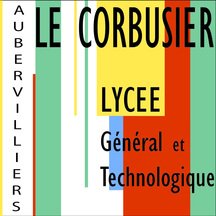
\includegraphics[width=0.18\linewidth]{corbu.jpg} \hspace{2.5cm} \normalsize \textsc{TP Industrialisation \hspace{2.5cm} 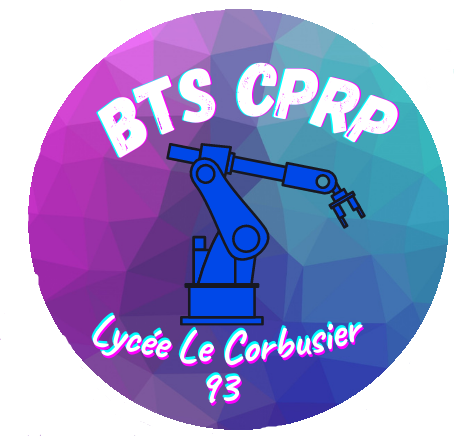
\includegraphics[width=0.2\linewidth]{btscprp.png}}
		\\ [2.0cm]
		\HRule{0.5pt} \\
		\LARGE \textbf{\uppercase{TP1.4 Axes Machines \& architecture des MOCN}}
		\HRule{2pt} \\ [0.5cm]}
\maketitle

\textbf{Deux personnes par groupe}\\


Nom :  \hspace{5cm} Prénom : \\


\vspace{1cm}

-----------------------------------  \hspace{1cm}   ---------------------------------

\vspace{1cm}

-----------------------------------  \hspace{1cm}   ---------------------------------




%\tableofcontents
%-------------------------------------------------------------------------------
% Section title formatting
\sectionfont{\scshape}




\newpage



%%%%%%%%%%%%%%%%%%%%%%%%%%%%%%%%%%%%%%%%%%%%%%%%%%%%%%%%%%%%%%%%
%%%%%%%%%%%%%%%% MACHINE 1 %%%%%%%%%%%%%%%%%%%%%%%%%%%%%%%%%%%%%
%%%%%%%%%%%%%%%%%%%%%%%%%%%%%%%%%%%%%%%%%%%%%%%%%%%%%%%%%%%%%%%%

Une machine outil à commande numérique, appelée communément MOCN, est un système
automatisé. Elle est composée d’une partie commande (PC) : le DCN (directeur de commande
numérique) et d’une partie opérative (PO) comprenant la structure de la machine outil, le porte-outil, l’outil et le porte-pièce ; la matière d’oeuvre est la pièce.
\begin{figure}
\centering
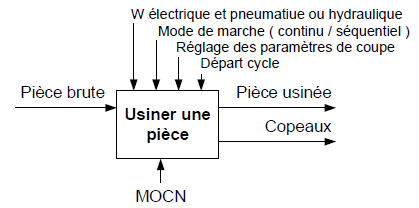
\includegraphics[width=0.7\linewidth]{A0.PNG}
\caption{Analyse fonctionnelle niveau A-0}
\label{A0}
\end{figure}
\section{Généralités sur les MOCN}
\textit{Savoir et connaissance du programme : S7.4.1 Caractéristiques des machines de production \& S7.4 – Machines}
\subsection{Machine 1}

\begin{exo}\label{exo1} A propos de la machine ci-dessous, rayer les mentions inutiles :
\begin{itemize}
    \item C'est une fraiseuse à commande numérique;
    \item C'est un tour à commande numérique;
    \item C'est une perceuse à colonne.
\end{itemize}
\end{exo}


\begin{exo}\label{exo1} Retrouvez les différentes axes, pièces et ensembles constituant la machine-outil à commande numérique (MOCN Figure \ref{MOCN11} \& \ref{MOCN12}) et indiquez les numéros correspondants :\\ \end{exo}
\begin{minipage}{.55\linewidth}
\begin{itemize}
    \item Outil numéro x :
    \item Broche :
    \item Arrosage :
    \item Arrêt d’urgence :
    \item Magasin d’outils :
    \item Directeur de commande numérique :
    \item Porte de sécurité :
\end{itemize}

\end{minipage}
\begin{minipage}{.44\linewidth}
\begin{itemize}
    \item Porte de sécurité :
    \item Bac à copeaux :
    \item Étau :
    \item Axe X :
    \item Outil :
    \item Axe Z :
    \item Bâti :
\end{itemize}
\end{minipage}

\begin{figure}
\centering
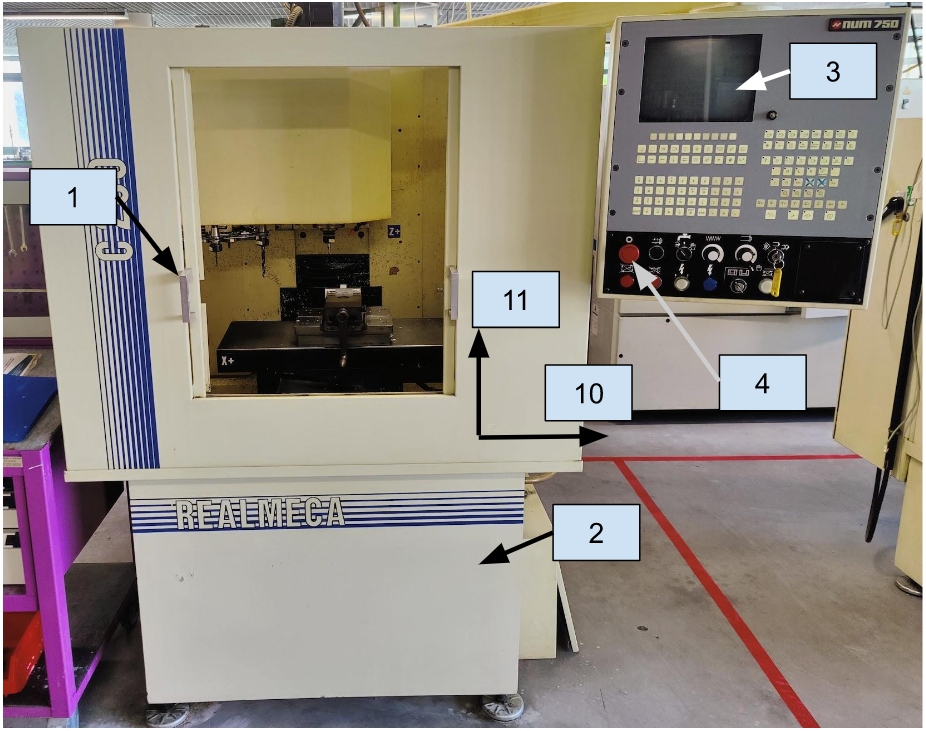
\includegraphics[width=0.7\linewidth]{MOCN11.PNG}
\caption{MOCN 1 - Extérieur}
\label{MOCN11}


\centering
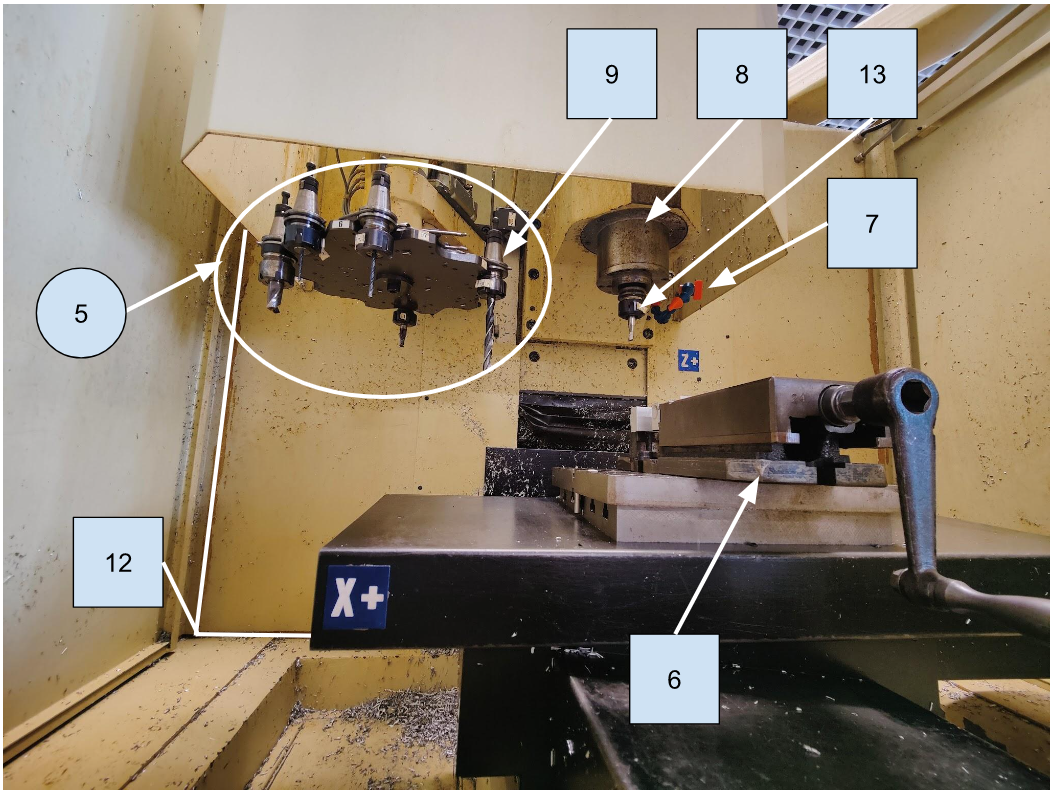
\includegraphics[width=0.7\linewidth]{MOCN12.PNG}
\caption{MOCN 1 - Intérieur}
\label{MOCN12}
\end{figure}



%%%%%%%%%%%%%%%%%%%%%% FIN %%%%%%%%%%%%%%%%%%%%%%%%%%%%%%%%%%%%%%%%%%%%%%
%%%%%%%%%%%%%%%%%%%%%%%%%%%%%%%%%%%%%%%%%%%%%%%%%%%%%%%%%%%%%%%%%%%%%%%%%




%%%%%%%%%%%%%%%%%%%%%%%%%%%%%%%%%%%%%%%%%%%%%%%%%%%%%%%%%%%%%%%%
%%%%%%%%%%%%%%%% MACHINE 2 %%%%%%%%%%%%%%%%%%%%%%%%%%%%%%%%%%%%%
%%%%%%%%%%%%%%%%%%%%%%%%%%%%%%%%%%%%%%%%%%%%%%%%%%%%%%%%%%%%%%%%




\subsection{Machine 2}

\begin{exo}\label{exo1} A propos de la machine ci-dessous, rayer les mentions inutiles :
\begin{itemize}
    \item C'est une fraiseuse à commande numérique;
    \item C'est un tour à commande numérique;
    \item C'est une perceuse à colonne.
\end{itemize}
\end{exo}


\begin{exo}\label{exo1} Retrouvez les différentes axes, pièces et ensembles constituant la machine-outil à commande numérique (MOCN Figure \ref{MOCN21} \& \ref{MOCN22}) et indiquez les numéros correspondants :\\ \end{exo}
\begin{minipage}{.55\linewidth}
\begin{itemize}
    \item Outil numéro x :
    \item Mors :
    \item Mandrin :
    \item Guide chariot vertical $\overrightarrow{x}$ :
    \item Contre-broche :
    \item Centre de commande / pupitre\\ de commande (IHM : Interface homme machine) :
    \item Porte de sécurité :
    \item Axe $\overrightarrow{X}$ :
    \item Bâti :
\end{itemize}


\end{minipage}
\begin{minipage}{.44\linewidth}
\begin{itemize}
    \item Magasin d’outils :
    \item Bac à copeaux :
    \item Marque du constructeur :
    \item Modèle du constructeur :
    \item Bouton d'arrêt d’urgence :
    \item Axe $\overrightarrow{Z}$ :
    \item Axe $\overrightarrow{C}$ :
    \item Axe $\overrightarrow{Y}$ :
\end{itemize}
\end{minipage}

\begin{figure}
\centering
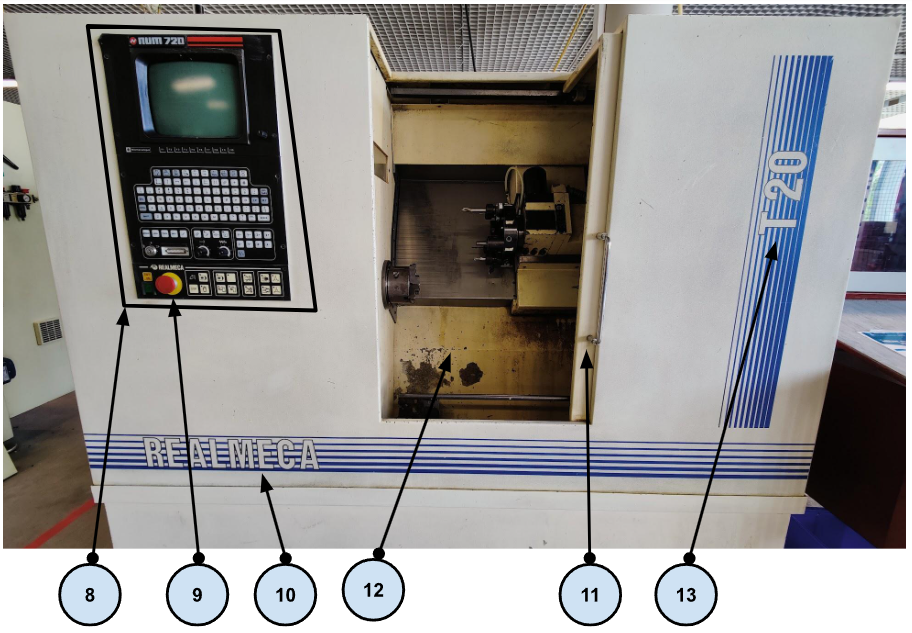
\includegraphics[width=0.75\linewidth]{MOCN21.PNG}
\caption{MOCN 2 - Extérieur}
\label{MOCN21}


\centering
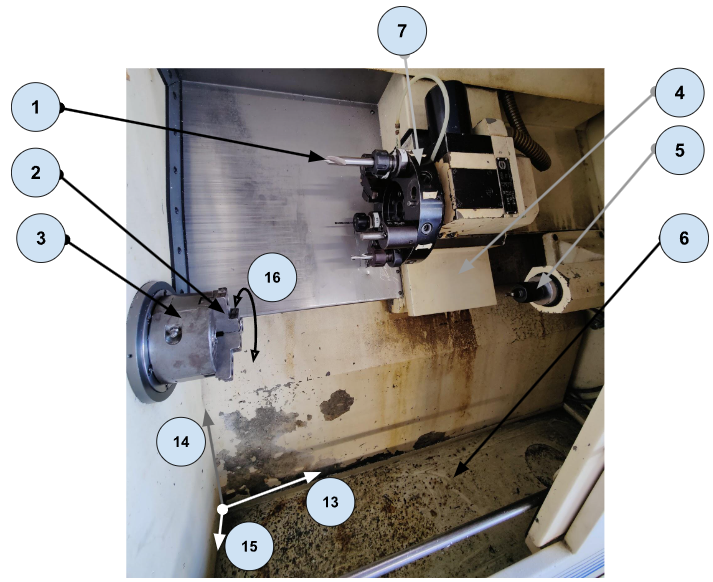
\includegraphics[width=0.75\linewidth]{MOCN22.PNG}
\caption{MOCN 2 - Intérieur}
\label{MOCN22}
\end{figure}
%%%%%%%%%%%%%%%%%%%%%% FIN %%%%%%%%%%%%%%%%%%%%%%%%%%%%%%%%%%%%%%%%%%%%%%
%%%%%%%%%%%%%%%%%%%%%%%%%%%%%%%%%%%%%%%%%%%%%%%%%%%%%%%%%%%%%%%%%%%%%%%%%




\newpage


\section{Fonctionnement des machines outils}
\textit{Compétence travaillée : S7.4 – Machines}

\begin{figure}
\centering
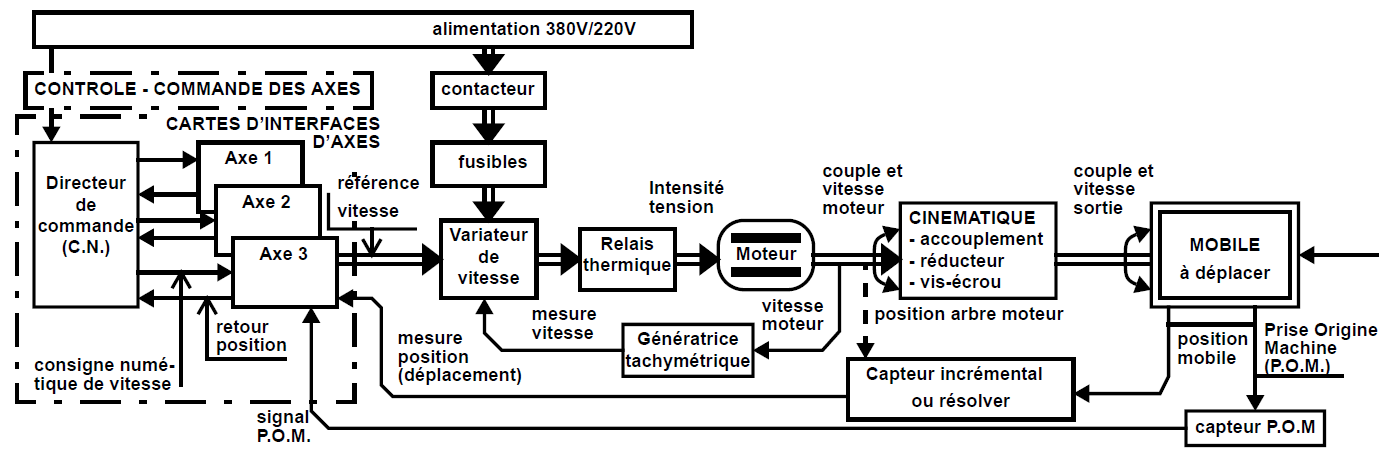
\includegraphics[width=1\linewidth]{fonction1.PNG}
\caption{Fonction contrôle / commande d’une commande d’axe. E.Duc \& E. Lefur.}
\label{F1}
\end{figure}

\begin{exo}\label{exo1} En vous aidant de la Figure \ref{F1} indiquez d'où viennent les ordres de déplacement des machines outils.\end{exo}
%% D'après la figure, les ordres viennent de la consigne de vitesse dans le directeur de commande (C.N.)

\begin{exo}\label{exo1} Selon le diagramme Figure \ref{F1} de combien d'axe(s) dispose la machine outil  ?\end{exo}
%% De trois axes %%

\begin{figure}
\centering
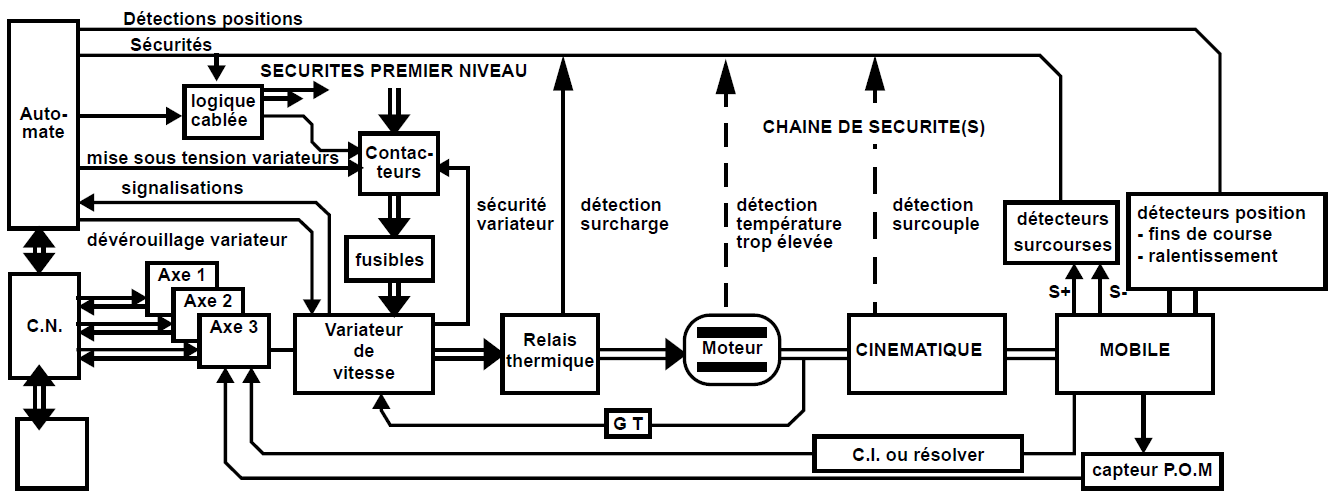
\includegraphics[width=1\linewidth]{conduite1.PNG}
\caption{Fonction conduite / surveillance d’une commande d’axe. E.Duc \& E. Lefur.}
\label{C1}
\end{figure}

\begin{exo}\label{exo1} En vous aidant de la Figure \ref{C1} : Que se passe-t-il si, lors d'une erreur de programmation d'usinage, un outil force sur la pièce ?\end{exo}
%% Si un outil force, le couple va augmenter jusqu'à détection du surcouple, la chaîne de sécurité sera alerté et l'automate,  par l'intermédiaire d'une signalisation et du contrôle du variateur, va pouvoir arrêter le processus en cours %%

\section{Structures \& architectures des machines outils}
\textit{Compétences travaillées :
\begin{itemize}
    \item S7.4.1 – Caractéristiques des machines de production ;
    \item S3.1 – Modélisation des mécanismes ;
    \item S11.1.3 – Structures sérielles et parallèles.
\end{itemize}
 }


La structure articulaire (voir Figure \ref{S1} et Figure \ref{S2}) est le squelette de la machine; il se trouve sous le carter et n'est pas accessible par l'utilisateur. Par analogie au corps humain, nous parlons du squelette de la machine. Ce squelette est composé en général de liaison à \textbf{1 degré de liberté} (articulation) de type \textbf{liaison pivot} (comme notre coude) ou \textbf{liaison glissière} (comme nous, dans un toboggan !).\\

Pour rappel, il existe différentes façon de structurer un système. Des exemples sont visibles sur les \textbf{Figures \ref{Se1}, Figure \ref{Par1}, Figure \ref{Par2} et Figure \ref{Par3}}.

\begin{exo}\label{exo1} En rappelant le nom des machines outils sur lesquelles vous vous êtes rendus, indiquez si, d'après vous, elles font partie d'une structure type \textbf{ouverte} ou \textbf{fermée}. Aidez vous des figures \ref{S1} \& \ref{S2}.\end{exo}

\begin{exo}\label{exo1} Appelez votre enseignant, et inspectez si dans l'atelier de production, vous disposez de machine avec une structure en parallèle.\end{exo}





\section{Système d'axe des machines outil}
% Aide question : http://philippe.berger2.free.fr/productique/ressources/origines/origines.htm %%%

%% https://fr.calameo.com/read/00087507071e3620cbe22 %%
%% https://fr.calameo.com/books/00087507071e3620cbe22 %%


\subsection{Définition}

\begin{exo}\label{exo1} Rappelez l'intérêt des normes dans l'industrie.\end{exo}


\begin{exo}\label{exo1} Recherchez la définition de la norme \textbf{AFNOR NF Z 68-020}, quel est son but ?\end{exo}







\subsection{Butées des axes machines}





%%%%%%%%%%%%%%%%%%%%%%%%%%%%%%%%%%%%%%%%%%%%%%%%%%%%%%%%%%%%%%%%%%%%%%%%%%%%%%%%%%%%%%
%%%%%%%%%%%%%%%%%%%%%%%%%%%%%%%%%%%%%%%%%%%%%%%%%%%%%%%%%%%%%%%%%%%%%%%%%%%%%%%%%%%%%%
%%%%%%%%%%%%%%%%%%%%%%%%%%%%%%%%%%%%%%%%%%%%%%%%%%%%%%%%%%%%%%%%%%%%%%%%%%%%%%%%%%%%%%



%%%%%%%%%%%%%%%%%%%%%%%%%%%%%%%%%%%%%%%%%%%%%%%%%%%%%%%%%%%%%%%%%%%%%%%%%%%%%%%%%%%%%%
%%%%%%%%%%%%%%%%%%%%%%%%%%%%%%%%%%%%%%%%%%%%%%%%%%%%%%%%%%%%%%%%%%%%%%%%%%%%%%%%%%%%%%
%%%%%%%%%%%%%%%%%%%%%%%%%%%%%%%%%%%%%%%%%%%%%%%%%%%%%%%%%%%%%%%%%%%%%%%%%%%%%%%%%%%%%%

\section{ANNEXE}
\begin{figure}
\begin{minipage}{.55\linewidth}

\centering
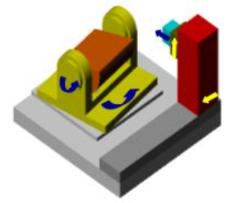
\includegraphics[width=0.7\linewidth]{S1.PNG}
\caption{Exemple 1 : Centre d'usinage 5 axes, structure à type ouverte.}
\label{S1}

\end{minipage}
\begin{minipage}{.44\linewidth}

\centering
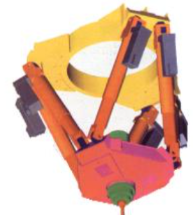
\includegraphics[width=0.7\linewidth]{S2.PNG}
\caption{Exemple 2 : Centre d'usinage 5 axes, structure à type fermée.}
\label{S2}

\end{minipage}
\end{figure}

%%%%%%%%%%%%%%%%%%%%%%%%%%%%%%%%%%%%%%%%%%%%%%%%%%%%%%%%%%%%%%%%%%%%%%%%%%%%%%%%%%%%%%
%%%%%%%%%%%%%%%%%%%%%%%%%%%%%%%%%%%%%%%%%%%%%%%%%%%%%%%%%%%%%%%%%%%%%%%%%%%%%%%%%%%%%%
%%%%%%%%%%%%%%%%%%%%%%%%%%%%%%%%%%%%%%%%%%%%%%%%%%%%%%%%%%%%%%%%%%%%%%%%%%%%%%%%%%%%%%


\begin{figure}
\centering
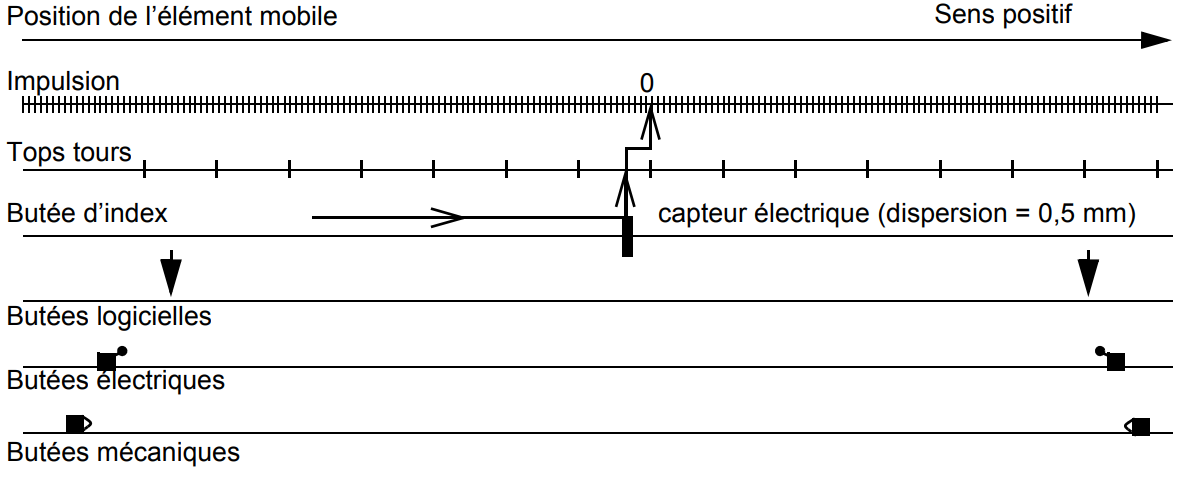
\includegraphics[width=0.85\linewidth]{pos1.PNG}
\caption{Procédure d’initialisation d’un axe numérique pour la prise d'origine machine (POM) (Etienne LEFUR et Christophe SOHIER - Ecole Normale Supérieure de CACHAN.)}
\label{m2}
\end{figure}

%%%%%%%%%%%%%%%%%%%%%%%%%%%%%%%%%%%%%%%%%%%%%%%%%%%%%%%%%%%%%%%%%%%%%%%%%%%%%%%%%%%%%%
%%%%%%%%%%%%%%%%%%%%%%%%%%%%%%%%%%%%%%%%%%%%%%%%%%%%%%%%%%%%%%%%%%%%%%%%%%%%%%%%%%%%%%
%%%%%%%%%%%%%%%%%%%%%%%%%%%%%%%%%%%%%%%%%%%%%%%%%%%%%%%%%%%%%%%%%%%%%%%%%%%%%%%%%%%%%%


\begin{figure}
\begin{minipage}{.55\linewidth}

\centering
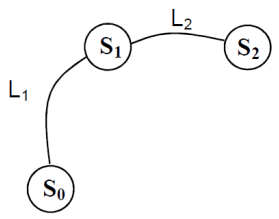
\includegraphics[width=0.7\linewidth]{serie1.PNG}
\caption{Exemple 1.1 : Chaîne de solide en série ouverte.}
\label{Se1}

\end{minipage}
\begin{minipage}{.44\linewidth}

\centering
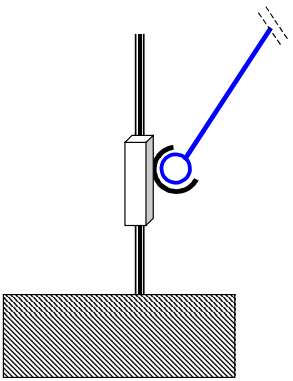
\includegraphics[width=0.7\linewidth]{par1.PNG}
\caption{Exemple 1.2 : Schéma cinématique en série.}
\label{Par1}

\end{minipage}
\end{figure}


%%%%%%%%%%%%%%%%%%%%%%%%%%%%%%%%%%%%%%%%%%%%%%%%%%%%%%%%%%%%%%%%%%%%%%%%%%%%%%%%%%%%%%
%%%%%%%%%%%%%%%%%%%%%%%%%%%%%%%%%%%%%%%%%%%%%%%%%%%%%%%%%%%%%%%%%%%%%%%%%%%%%%%%%%%%%%
%%%%%%%%%%%%%%%%%%%%%%%%%%%%%%%%%%%%%%%%%%%%%%%%%%%%%%%%%%%%%%%%%%%%%%%%%%%%%%%%%%%%%%


\begin{figure}
\begin{minipage}{.55\linewidth}

\centering
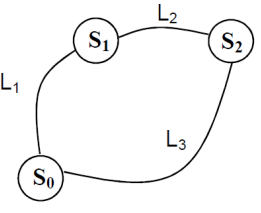
\includegraphics[width=0.7\linewidth]{par2.PNG}
\caption{Exemple 2.1 : Chaîne de solide en parallèle fermée.}
\label{Par2}

\end{minipage}
\begin{minipage}{.44\linewidth}

\centering
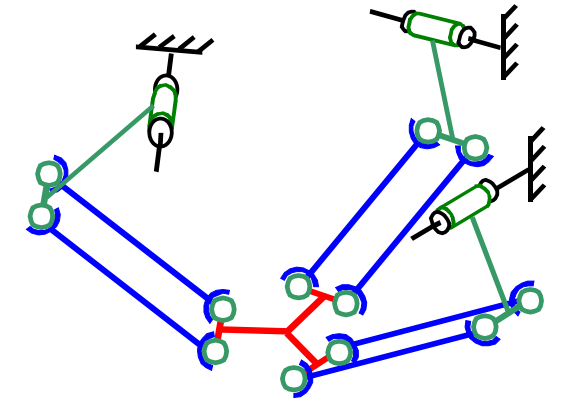
\includegraphics[width=0.8\linewidth]{par3.PNG}
\caption{Exemple 2.2 : Schéma cinématique en parallèle fermée.}
\label{Par3}

\end{minipage}
\end{figure}

%%%%%%%%%%%%%%%%%%%%%%%%%%%%%%%%%%%%%%%%%%%%%%%%%%%%%%%%%%%%%%%%%%%%%%%%%%%%%%%%%%%%%%
%%%%%%%%%%%%%%%%%%%%%%%%%%%%%%%%%%%%%%%%%%%%%%%%%%%%%%%%%%%%%%%%%%%%%%%%%%%%%%%%%%%%%%
%%%%%%%%%%%%%%%%%%%%%%%%%%%%%%%%%%%%%%%%%%%%%%%%%%%%%%%%%%%%%%%%%%%%%%%%%%%%%%%%%%%%%%










%%%%%%%%%%%%%%%%%%%%%%%%%%%%%%%%%%%%%%%%%%%%%%%%%%%%%%%%%%%%%%%%%%%%%%%%%%%%%%%%%%%%%%
%%%%%%%%%%%%%%%%%%%%%%%%%%%%%%%%%%%%%%%%%%%%%%%%%%%%%%%%%%%%%%%%%%%%%%%%%%%%%%%%%%%%%%
%%%%%%%%%%%%%%%%%%%%%%%%%%%%%%%%%%%%%%%%%%%%%%%%%%%%%%%%%%%%%%%%%%%%%%%%%%%%%%%%%%%%%%


%%%%%%%%%%%%%%%%%%%%%%%%%%%%%%%%%%%%%%%%%%%%%%%%%%%%%%%%%%%%%%%%%%%%%%%%%%%%%%%%%%%%%%
%%%%%%%%%%%%%%%%%%%%%%%%%%%%%%%%%%%%%%%%%%%%%%%%%%%%%%%%%%%%%%%%%%%%%%%%%%%%%%%%%%%%%%
%%%%%%%%%%%%%%%%%%%%%%%%%%%%%%%%%%%%%%%%%%%%%%%%%%%%%%%%%%%%%%%%%%%%%%%%%%%%%%%%%%%%%%


%%%%%%%%%%%%%%%%%%%%%%%%%%%%%%%%%%%%%%%%%%%%%%%%%%%%%%%%%%%%%%%%%%%%%%%%%%%%%%%%%%%%%%
%%%%%%%%%%%%%%%%%%%%%%%%%%%%%%%%%%%%%%%%%%%%%%%%%%%%%%%%%%%%%%%%%%%%%%%%%%%%%%%%%%%%%%
%%%%%%%%%%%%%%%%%%%%%%%%%%%%%%%%%%%%%%%%%%%%%%%%%%%%%%%%%%%%%%%%%%%%%%%%%%%%%%%%%%%%%%








\end{document}

